%%%%%%%%%%%%%%%%%%%%%%%%%%%%%%%%%%%%%%%%%%%%%%%%%%%%%%%%%%%%%%%%%%%%%%%%%%
%%%%%                         CHAPITRE 3                            %%%%%%
%%%%%%%%%%%%%%%%%%%%%%%%%%%%%%%%%%%%%%%%%%%%%%%%%%%%%%%%%%%%%%%%%%%%%%%%%%

\lhead[\fancyplain{}{\leftmark}]%Pour les pages paires \bfseries
      {\fancyplain{}{}} %Pour les pages impaires
\chead[\fancyplain{}{}]%
      {\fancyplain{}{}}
\rhead[\fancyplain{}{}]%Pour les pages paires 
      {\fancyplain{}{\rightmark}}%Pour les pages impaires \bfseries
\lfoot[\fancyplain{}{}]%
      {\fancyplain{}{}}
\cfoot[\fancyplain{}{\thepage}]%\bfseries
      {\fancyplain{}{\thepage}} %\bfseries
\rfoot[\fancyplain{}{}]%
     {\fancyplain{}{\scriptsize}}


%%%%%%%%%%%%%%%%%%%%%%%%%%%%%%%%%%%%%%%%%%%%%%%%%%%%%%%%%%%%%%%%%%%%%%%%%%
%%%%%                      Start part here                          %%%%%%
%%%%%%%%%%%%%%%%%%%%%%%%%%%%%%%%%%%%%%%%%%%%%%%%%%%%%%%%%%%%%%%%%%%%%%%%%%

\chapter{Proposed solution: Pose2Sim Python package}
\label{ch:3}

%==============================================================================	Résumé du chapitre

\begin{center}
\rule{0.7\linewidth}{.5pt}
\begin{minipage}{0.7\linewidth}
\smallskip

\textit{We propose the Pose2Sim python package, as an alternative to the more usual marker-based motion capture methods.Pose2Sim stands for "OpenPose to OpenSim", as it uses OpenPose inputs (2D keypoints coordinates obtained from multiple videos) and leads to an OpenSim result (physically consistent full-body 3D joint angles). Code is available at \url{https://github.com/perfanalytics/pose2sim}. \newline \newline
This chapter is adapted from the article published in the Journal of Open Source Software: "Pose2Sim: An Open-source Python Package for multiview markerless kinematics" \cite{Pagnon2022b}.}

%\smallskip
\end{minipage}
\smallskip
\rule{0.7\linewidth}{.5pt}
\end{center}

\pagebreak
\minitoc

\vspace*{3cm}

\begin{figure}[hbtp]
	\centering
	\def\svgwidth{1\columnwidth}
	\fontsize{10pt}{10pt}\selectfont
	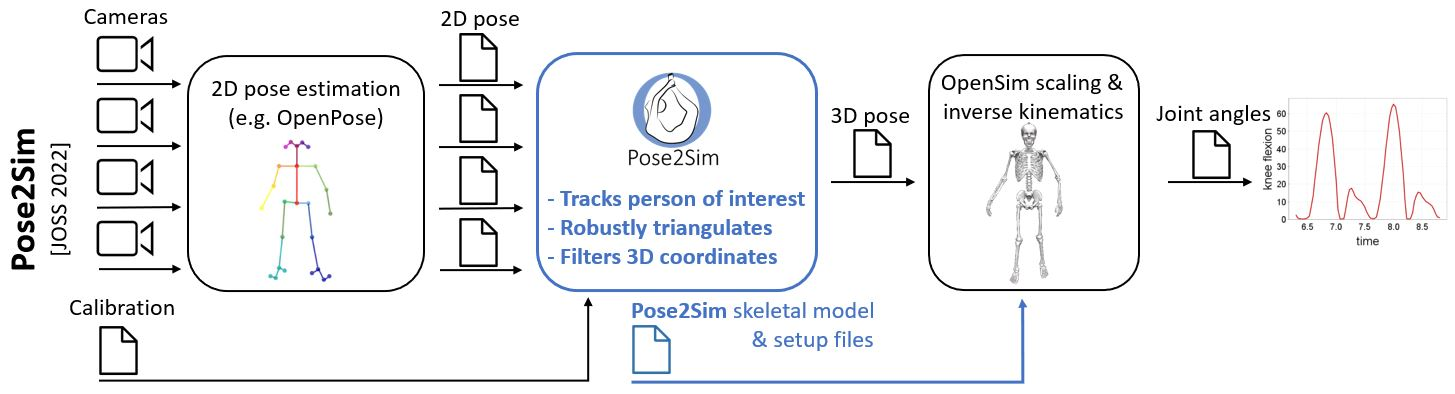
\includegraphics[width=\linewidth]{"../Intro/Figures/Fig_VisAbstract1.JPG"}
      \caption{Visual abstract for the Pose2Sim workflow \cite{Pagnon2022b}.}
	\label{fig_visabstract1}
\end{figure}

\newpage


\section{Introduction to the workflow}

Although some developments are relevant to both, specifics differ between medicine and the sports field. In this regard and as stated in the \nameref{sec:statement of need}, marker-based methods are not well suited for sports motion analysis \cite{Colyer2018}. In sports, capture should not hinder the movement. Placing markers on the naked body takes time and is cumbersome, therefore markerless approaches are favored. Sports environments are usually much more challenging than lab settings: frequent occlusions, fast and unusual movements, and complex background make it important to resort to using multiple view points, from RGB rather than RGB-D cameras, processed with machine learning methods. Competition conditions are often fast-paced and congested, so a light-weight, fast, and easy to set up system is relevant. However, as coaches and athletes usually need a mere feedback rather than a definitive diagnosis, they don't need as thorough of an accuracy as physicians. Ideally, results should be given in real time, and they should be more visual than graphs of time series. Moreover, 3D kinematics are more relevant than 2D sagittal plane kinematics; and full-body analysis (including upper-limb) is desired.

We propose the Python package Pose2Sim \cite{Pagnon2022b}, which aims to deal with these constraints. It provides a framework for 3D markerless kinematics, as an alternative to the more usual marker-based motion capture methods. Pose2Sim stands for "OpenPose to OpenSim", as it uses OpenPose inputs (2D coordinates obtained from multiple videos) \cite{Cao2019} and leads to an OpenSim result (full-body 3D joint angles) \cite{Delp2007,Seth2018}. Pose2Sim is accessible at \url{https://github.com/perfanalytics/pose2sim}.

\begin{figure}[hbtp]
	\centering
	\def\svgwidth{1\columnwidth}
	\fontsize{10pt}{10pt}\selectfont
	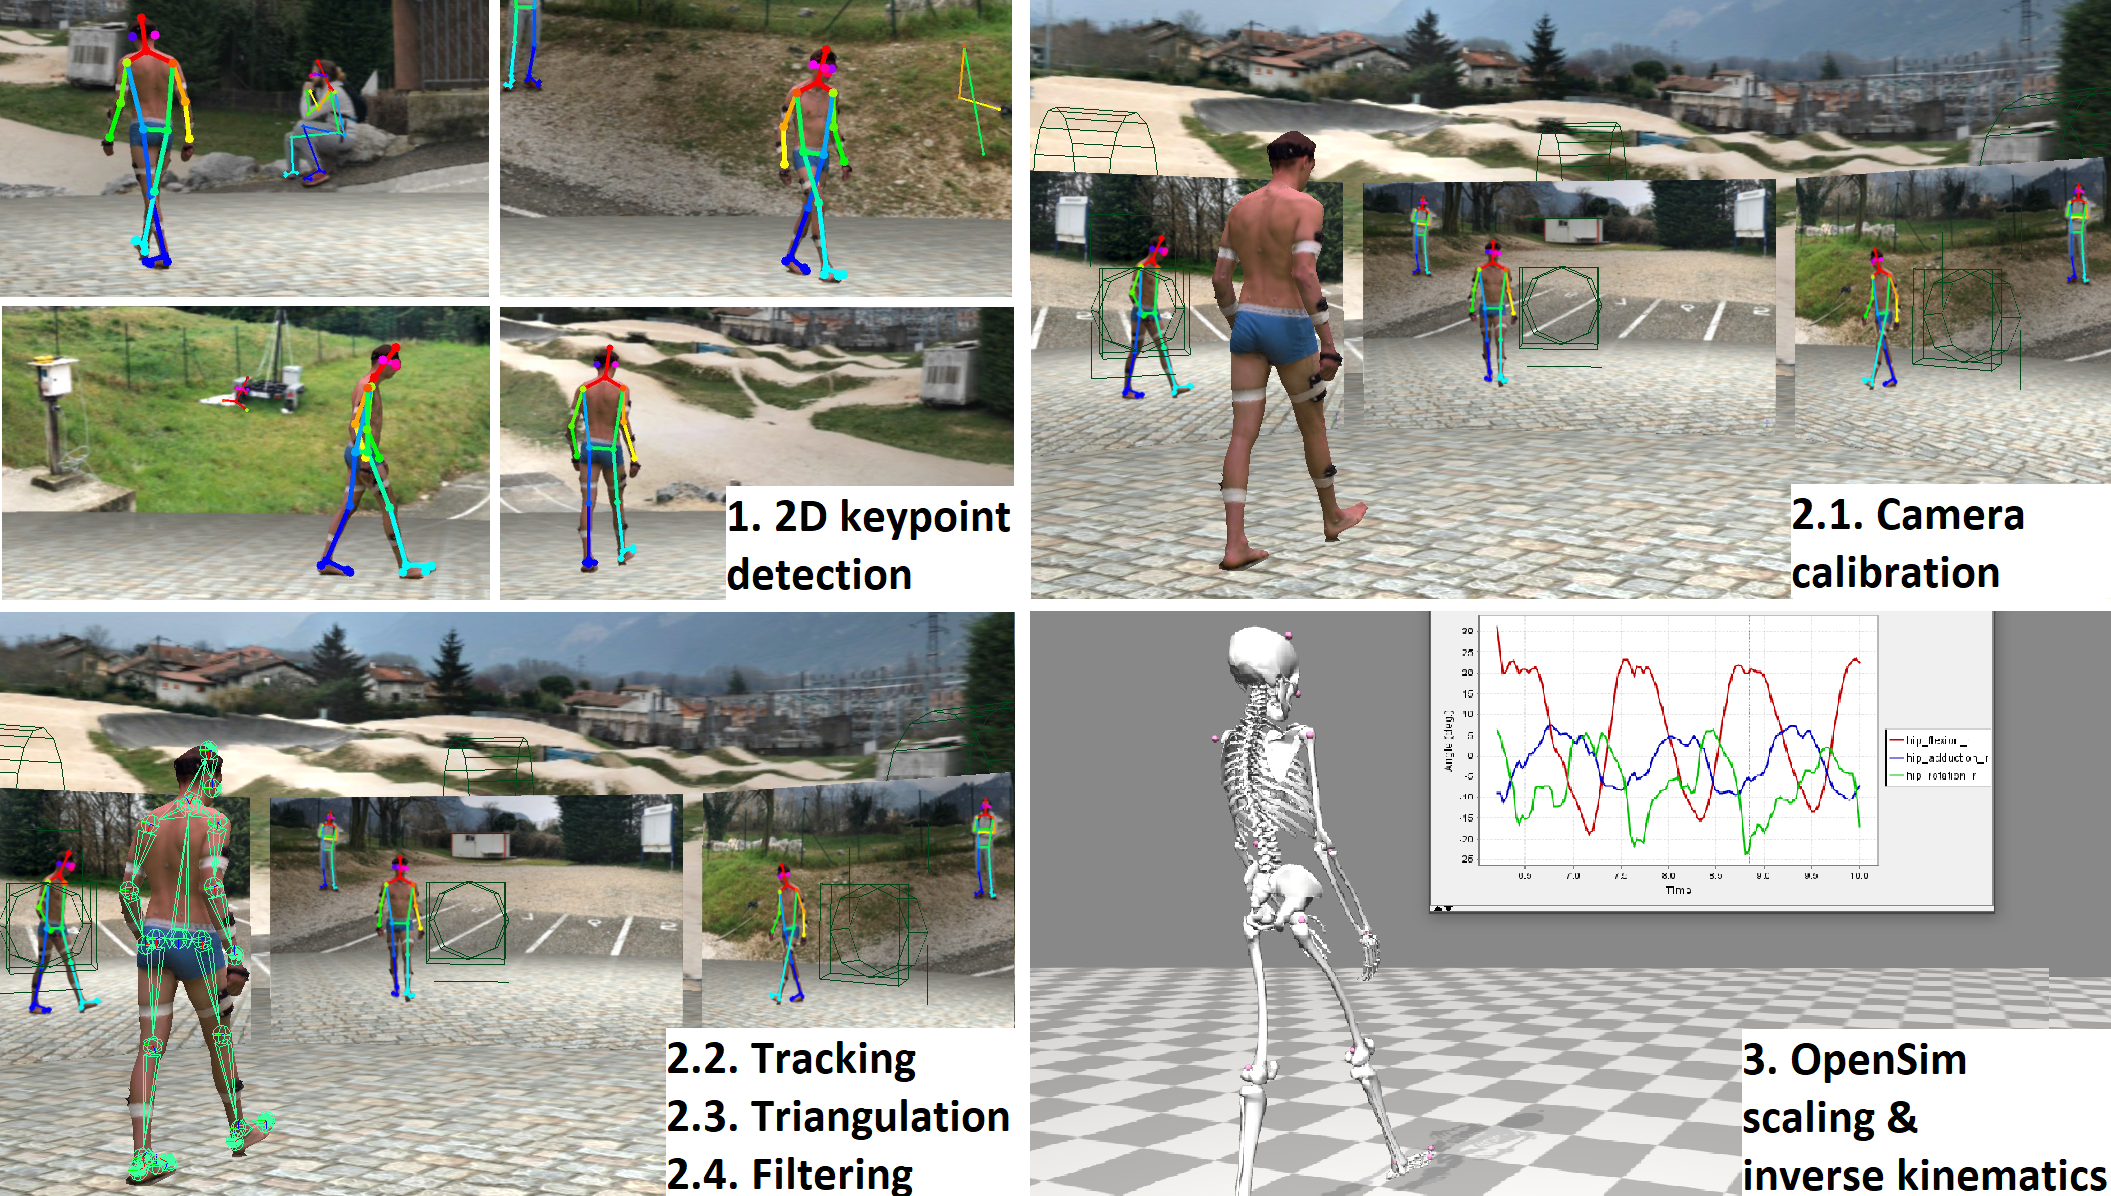
\includegraphics[width=\linewidth]{"../Chap3/Figures/Fig_Pipeline.png"}
	\caption{Pose2Sim full pipeline: (1) 2D keypoint detection; (2.1) Camera calibration; \newline(2.1-2.4) Tracking of the person of interest, Triangulating of keypoint coordinates; and Filtering; (3) Constraining the 3D coordinates to an individually scaled, physically consistent OpenSim skeletal model.}
	\label{fig_pipeline}
\end{figure}

\newpage

The repository presents a framework which consists in (Figures~\ref{fig_pipeline}):
\begin{enumerate}[itemsep=0em, topsep=0em, leftmargin=*]
      \item Preliminary 2D joint coordinate detections from multiple videos, e.g. with OpenPose.
      \item Pose2Sim core, including 4 customizable steps:
      \begin{enumerate}[before=\vspace{-0.5\baselineskip}, nosep, label*=\arabic*.]
            \item Camera calibration.
            \item 2D tracking of the person of interest.
            \item 3D keypoint triangulation.
            \item 3D coordinate filtering.
      \end{enumerate}
      \item Scaling a full-body skeleton to each individual subject, and computing inverse kinematics via OpenSim so as to obtain 3D joint angles.
\end{enumerate}

\vskip 1em

Each task is easily customizable, and requires only moderate Python skills. The whole workflow runs from any video cameras, on any computer, equipped with any operating system (although OpenSim has to be compiled from source on Linux.) It requires no marker placement, and the scaling and inverse kinematic steps are simpler than they are with markers-based methods. Overall, human intervention is scarce, which makes it more robust to human error. Pose2Sim has already been used and tested in a number of situations (walking, running, cycling, dancing, balancing, swimming, boxing), and published in peer-reviewed scientific publications assessing the quality of its code \cite{Pagnon2022c}, its robustness (see Chapter 4 on \nameref{ch:4}) \cite{Pagnon2021} and its accuracy (see Chapter 5 on \nameref{ch:5}) \cite{Pagnon2022a}. Its results for inverse kinematics were deemed good when compared to marker-based ones, with errors generally below 4.0° across several activities, on both lower and on upper limbs. The combination of its ease of use, customizable parameters, and high robustness and accuracy makes it promising, especially for "in-the-wild" sports movement analysis.


\section{Installation and demonstration}

\subsection{Installation}

\begin{enumerate}[itemsep=0em, topsep=0em, leftmargin=*]
      \item Install \textbf{OpenPose} (instructions \href{https://github.com/CMU-Perceptual-Computing-Lab/openpose/blob/master/doc/installation/0_index.md}{here}).\newline
      Windows portable demo is enough.
      \item Install \textbf{OpenSim 4.x} from \href{https://simtk.org/frs/index.php?group_id=91}{there}.\newline
      Tested up to v4.4-beta on Windows. Has to be compiled from source on Linux (see \href{https://simtk-confluence.stanford.edu:8443/display/OpenSim/Linux+Support}{there}.
      \item \textit{Optional:} Install \textbf{Anaconda} or \href{https://docs.conda.io/en/latest/miniconda.html}{Miniconda}.\newline
      Open an Anaconda terminal and create a virtual environment by typing:
      \begin{minted}[frame=single, rulecolor=\color{gray!40}, autogobble]{shell-session}
            conda create -n Pose2Sim python=3.8.8
            conda activate Pose2Sim
      \end{minted}
      \item Install \textbf{Pose2Sim}\newline
      If you don't use Anaconda, type \mintinline{shell-session}{python -V} in terminal to make sure python>=3.6 is installed.
      \begin{itemize}
            \item OPTION 1: \textit{Quick install.} Type in terminal:
            \begin{minted}[frame=single, rulecolor=\color{gray!40}, autogobble]{shell-session}
                  pip install pose2sim
            \end{minted}
            \item OPTION 2: \textit{Build from source.} Open a terminal in the directory of your choice and clone the Pose2Sim repository:
            \begin{minted}[frame=single, rulecolor=\color{gray!40}, autogobble]{shell-session}
                  git clone https://gitlab.inria.fr/perfanalytics/pose2sim.git
                  cd pose2sim
                  pip install .
            \end{minted}
      \end{itemize}
\end{enumerate}


\subsection{Demonstration Part-1: Build 3D TRC file on Python}

This demonstration provides an example experiment of a person balancing on a beam, filmed with 4 calibrated cameras processed with OpenPose.

Open a terminal and check package location with  \mintinline{shell-session}{pip show pose2sim | grep Location}. \newline
Copy this path and go to the Demo folder with  \mintinline{shell-session}{cd <path>\pose2sim\Demo`}. \newline
Type \mintinline{shell-session}{python}, and test the following code (Figures~\ref{fig_pose2sim}):
\begin{minted}[frame=single, rulecolor=\color{gray!40}, autogobble]{python}
      from Pose2Sim import Pose2Sim
      Pose2Sim.calibrateCams()
      Pose2Sim.track2D()
      Pose2Sim.triangulate3D()
      Pose2Sim.filter3D()
\end{minted}

You should obtain a plot of all the 3D coordinates trajectories (Figures~\ref{fig_filterplot}). You can check the logs in \mintinline{shell-session}{Demo\Users\logs.txt}. Results are stored as .trc files in the \mintinline{shell-session}{Demo\pose-3d} directory (Figures~\ref{fig_trc}). Note that when the functions are called without any argument, the Config file is searched in the default \mintinline{shell-session}{Users\Config.toml} location. These parameters can be edited by the user.

\begin{figure}[hbtp]
	\centering
	\def\svgwidth{1\columnwidth}
	\fontsize{10pt}{10pt}\selectfont
	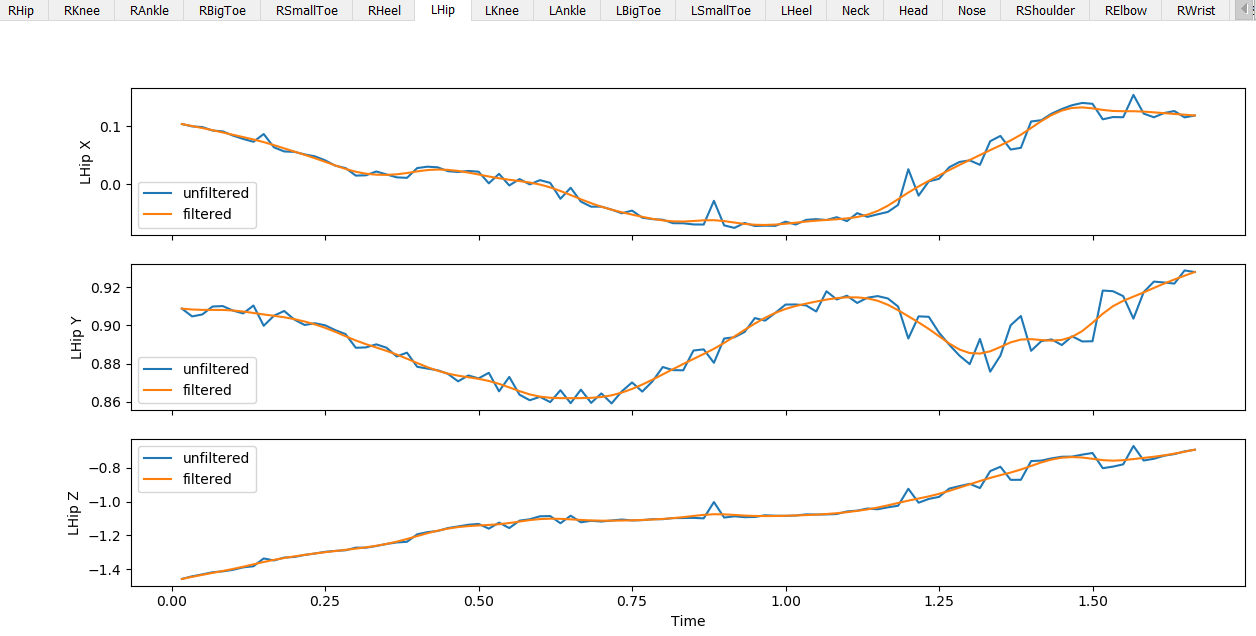
\includegraphics[width=\linewidth]{"../Chap3/Figures/Fig_FilterPlot.png"}
	\caption{Filtered results. Each keypoint trajectory is displayed in a different tab.}
	\label{fig_filterplot}
\end{figure}

\begin{figure}[hbtp]
	\centering
	\def\svgwidth{1\columnwidth}
	\fontsize{10pt}{10pt}\selectfont
	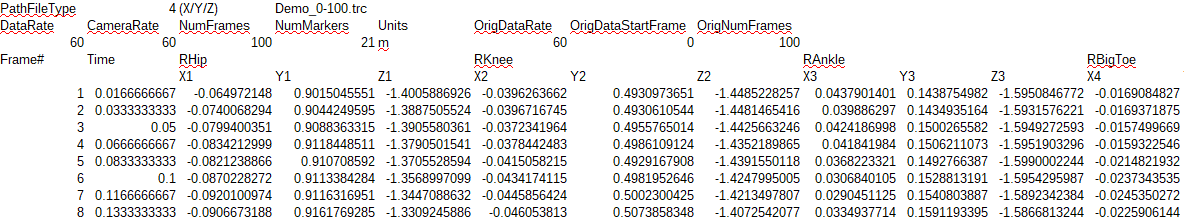
\includegraphics[width=\linewidth]{"../Chap3/Figures/Fig_Trc.png"}
	\caption{An example .trc file of triangulated keypoint coordinates, directly usable in OpenSim.}
	\label{fig_trc}
\end{figure}

\begin{figure}[hbtp]
	\centering
	\begin{subfigure}[b]{1\textwidth}
		\centering
		\def\svgwidth{\columnwidth}
		\fontsize{10pt}{10pt}\selectfont
		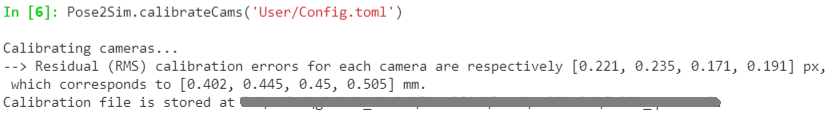
\includegraphics[width=\linewidth]{"../Chap3/Figures/Fig_Calib2D.png"}
            \caption{Calibration can either be done from a checkerboard, or by simply converting a Qualisys calibration file. Calibration errors are computed and provided.\newline}
      \end{subfigure}
	\qquad
	\begin{subfigure}[b]{1\textwidth}
		\centering
		\def\svgwidth{\columnwidth}
		\fontsize{10pt}{10pt}\selectfont
		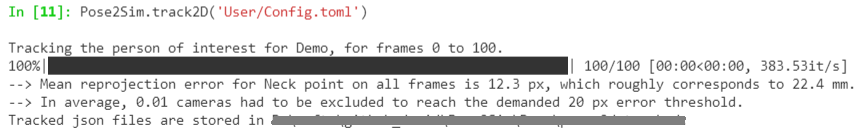
\includegraphics[width=\linewidth]{"../Chap3/Figures/Fig_Track2D.png"}
            \caption{If several persons are detected in the scene, a tracking step can be carried out in order to make sure that the right person from each camera will be triangulated.}
      \end{subfigure}
      \begin{subfigure}[b]{1\textwidth}
		\centering
		\def\svgwidth{1\columnwidth}
		\fontsize{10pt}{10pt}\selectfont
		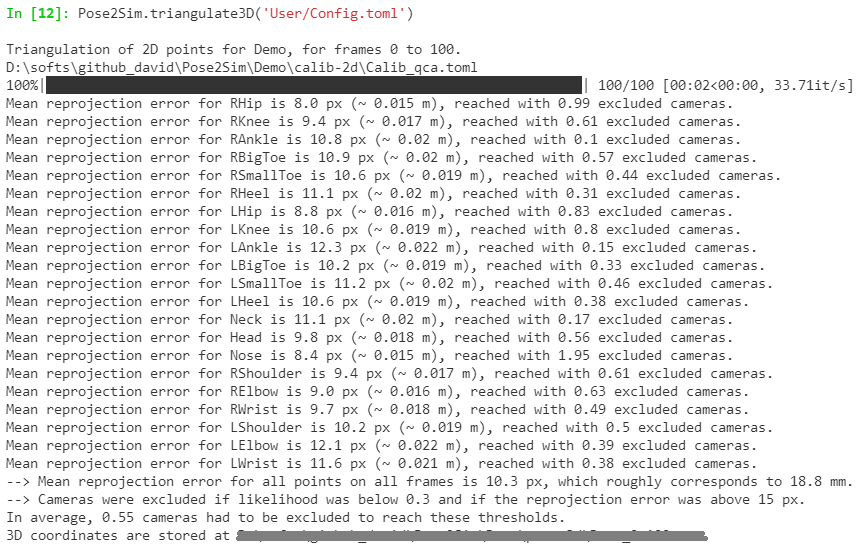
\includegraphics[width=\linewidth]{"../Chap3/Figures/Fig_Triangulate3D.png"}
            \caption{The triangulation is weighted by the OpenPose likelihood, and constrained by some thresholds defined in the Config.toml file. If these constraints are not met, e.g., if the reprojection error is too large or if the likelihood of a keypoint is too low, one or several cameras are excluded. The mean reprojection error and the number of cameras that have been excluded to meet the constraints is printed, for each keypoints.}
      \end{subfigure}
      \begin{subfigure}[b]{1\textwidth}
		\centering
		\def\svgwidth{1\columnwidth}
		\fontsize{10pt}{10pt}\selectfont
		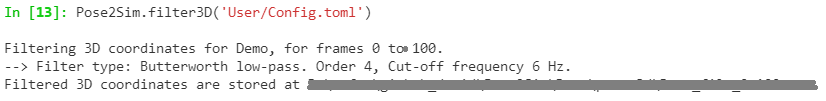
\includegraphics[width=\linewidth]{"../Chap3/Figures/Fig_Filter3D.png"}
            \caption{Triangulated data can be filtered, either with a low-pass Butterworth filter or with other types, and parameters can be adjusted.}
      \end{subfigure}
	\caption{First steps of Pose2Sim pipeline in Python. Calibration can either be done from a checkerboard, or by simply converting a Qualisys calibration file. Note that the functions can be used without any arguments if the Config.toml file is left in the default location.}
	\label{fig_pose2sim}
\end{figure}


\FloatBarrier
\subsection{Demonstration Part-2: Obtain 3D joint angles with OpenSim}
In the same vein as we would do with marker-based kinematics, the model first needs to be scaled to each individual, and then inverse kinematics can be performed (Figures~\ref{fig_opensimdemo}).

\textbf{Scaling:}
\begin{enumerate}[itemsep=0em, topsep=0em, leftmargin=*]
      \item Open OpenSim.
      \item Open the provided \mintinline{shell-session}{Model_Pose2Sim_Body25b.osim} model from \mintinline{shell-session}{pose2sim/Demo/opensim}. (File $\mapsto$ Open Model)
      \item Load the provided \mintinline{shell-session}{Scaling_Setup_Pose2Sim_Body25b.xml} scaling file from \mintinline{shell-session}{pose2sim/Demo/opensim}. (Tools $\mapsto$ Scale model $\mapsto$ Load)
      \item Run. You should see your skeletal model take the static pose.
\end{enumerate}

\textbf{Inverse kinematics}
\begin{enumerate}[itemsep=0em, topsep=0em, leftmargin=*]
    \item Load the provided \mintinline{shell-session}{IK_Setup_Pose2Sim_Body25b.xml} scaling file from \mintinline{shell-session}{pose2sim/Demo/opensim}. (Tools $\mapsto$ Inverse kinematics $\mapsto$ Load)
    \item Run. You should see your skeletal model move in the Vizualizer window.
\end{enumerate}

\begin{figure}[hbtp]
	\centering
	\def\svgwidth{1\columnwidth}
	\fontsize{10pt}{10pt}\selectfont
	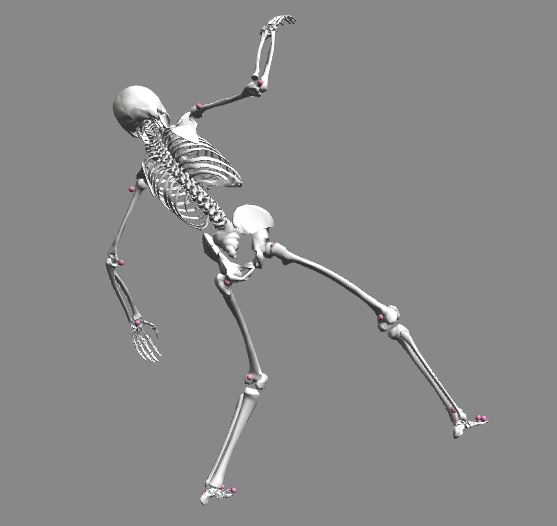
\includegraphics[width=\linewidth]{"../Chap3/Figures/Fig_OpenSimDemo.JPG"}
	\caption{At the end of the demonstration, you should have a skeleton balancing on a beam in OpenSim.}
	\label{fig_opensimdemo}
\end{figure}


\section{Method details}\label{methods_details}

\subsection{Project}
Pose2Sim is meant to be as fully and easily configurable as possible, by editing the \mintinline{shell-session}{User/Config.toml} file. First of all, the user can specify the project path and folder names, the video frame rate, and the range of analyzed frames. 

Optional tools are also provided for extending its usage (Figures~\ref{fig_opensimutilities}). Among others, DeepLabCut 2D files can be converted to the OpenPose formalism, and calibration files from other platforms can also be converted to the AniPose \cite{Karashchuk2021} formalism we use. 2D keypoint files can be displayed and stored as a video. Gait events can be detected from kinematic data thanks to \cite{Zeni2008} algorithm. Some other scripts allow for further processing of 3D coordinates. More practical information can be found on the GitHub repository. 

\begin{figure}[hbtp]
	\centering
	\def\svgwidth{1\columnwidth}
	\fontsize{10pt}{10pt}\selectfont
	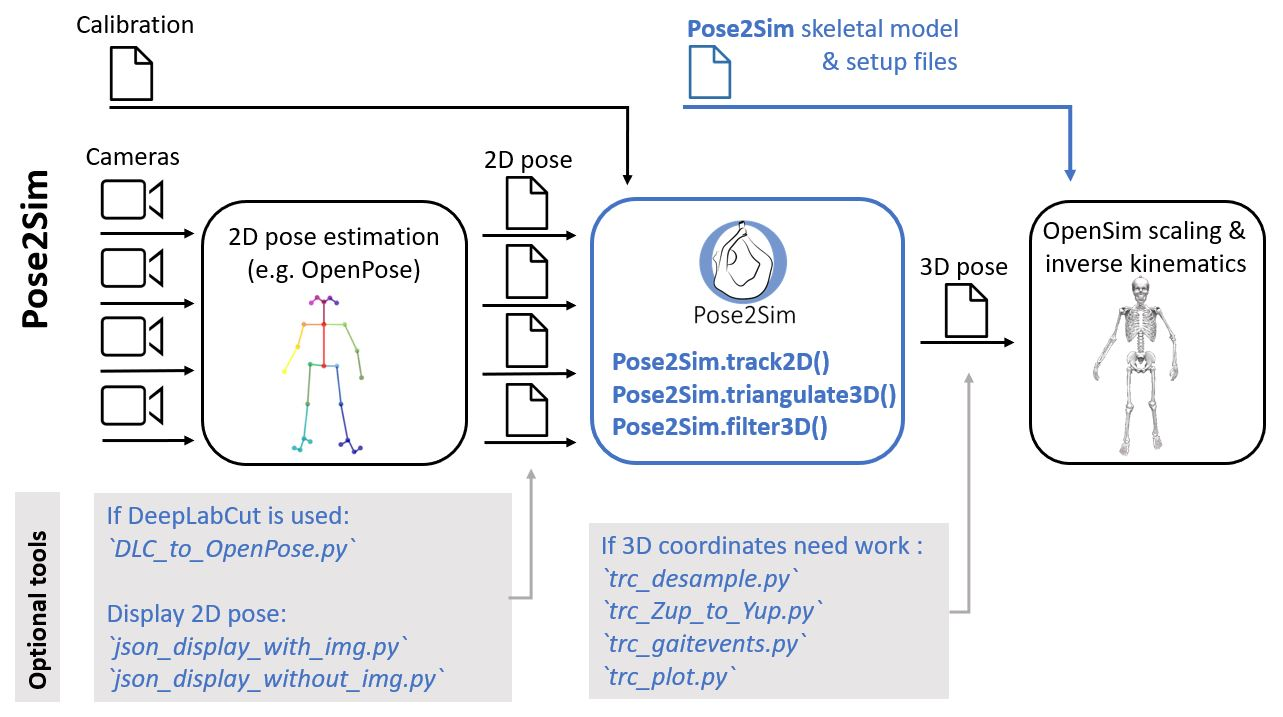
\includegraphics[width=\linewidth]{"../Chap3/Figures/Fig_Pose2SimUtilities.jpg"}
	\caption{The Pose2Sim workflow, along with some optional utilities provided in the package.}
	\label{fig_opensimutilities}
\end{figure}


\subsection{2D keypoint detection}

The interest in deep-learning pose estimation neural networks has been growing fast since 2015 \cite{Zheng2022}, which makes it now possible to collect accurate and reliable 2D landmark positions without the use of physical markers. OpenPose, for example, is a widespread open-source software which provides 2D joint coordinate estimates from videos. As it is the software we have extensively tested, we recommend choosing it.

Feet are usually needed in sports kinematic analysis, and OpenPose is one of the few programs which can detect them. Indeed, it comes with \{body + feet\} models such as body\_25 or body\_25B, as well as with a \{body + feet + hands + face\} one called body\_135 \cite{Hidalgo2019}. The latter two are more accurate than the standard body\_25 one. However, body\_135 requires high computational resources, unlike body\_25B which is as fast as body\_25, and which we have extensively tested \cite{Pagnon2022a}. Its keypoint definition differs slightly to the default model's (Figure~\ref{fig_body25b}): it adds the MPII head and neck keypoints, and removes the artificially created neck and middle hip points of the body\_25 model (which are simply the middle point of the shoulders and the hips). Hence, we recommend using it. Note that only 21 of the 25 detected keypoints are tracked, since eye and ear keypoints would be redundant in the determination of the head orientation. 

\begin{figure}[!ht]
	\centering
	\def\svgwidth{1\columnwidth}
	\fontsize{10pt}{10pt}\selectfont
	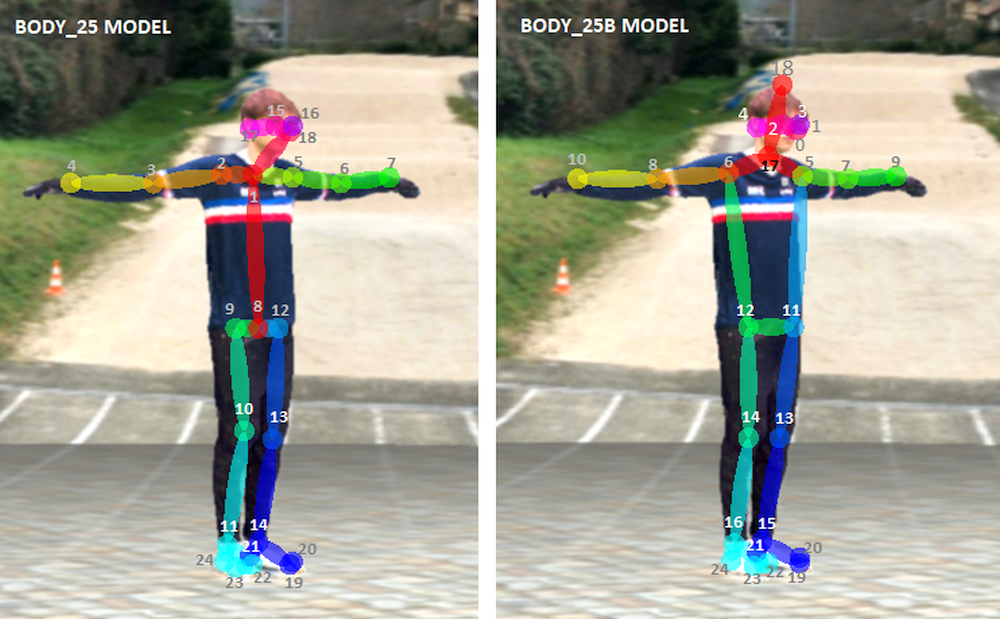
\includegraphics[width=\linewidth]{"../Chap3/Figures/Fig_Body25b.png"}
	\caption{The experimental body\_25b OpenPose model is more accurate than the default body\_25 one. See how the left knee is slightly misplaced on the default model. The keypoint definition differs between both models.}
	\label{fig_body25b}
\end{figure}

This being said, the user can choose any deep-learning pose estimation network. This choice will affect how keypoint indices will be mapped to model markers in OpenSim, corresponding to anatomical landmarks or joint centers. The OpenPose body\_25, body\_25B, body\_135, COCO, and MPII models are fully supported. The AlphaPose COCO, COCO-WholeBody, and full-body HALPE models are also supported, as well as the full-body but single-person detection BlazePose model. COCO and MPII model are the ones generally used by other networks such as OpenPifPaf \cite{Kreiss2021}, YOLO-pose \cite{Maji2022, Wang2022b}, and others, which means that they are also supported. It is also possible to build custom skeletons in the \mintinline{shell-session}{skeleton.py} file, trained for example with DeepLabCut \cite{Mathis2018, Lauer2022} or SLEAP \cite{Pereira2022}. They will be triangulated, but the user will need to build an OpenSim model and set the keypoints in the right place before being able to perform inverse kinematics.

%%%%%%%%%%%%%%%%%%%%%%%%%%%%%%%%%%%%%%%%%%%%%%%%%%%%%%%%%%%%%%%%%%%
% ATTENTION:                                                      %
% IMPLEMENTER CES MODELES ET LES TESTER AVANT DE PUBLIER LA THESE %
%%%%%%%%%%%%%%%%%%%%%%%%%%%%%%%%%%%%%%%%%%%%%%%%%%%%%%%%%%%%%%%%%%%
% OpenPose body_25b, OpenPose body_25, OpenPose body_135, AlphaPose HALPE_26, AlphaPose HALPE_136, AlphaPose COCO-WholeBody, MediaPipe BlazePose, COCO, MPII
% Convert SLEAP to OpenPose

Two optional standalone scripts are also provided if the user desires a visual display of the 2D pose estimation, as well as a tool for converting DeepLabCut data to OpenPose formalism (Figure~\ref{fig_opensimutilities}).


\subsection{Camera calibration}

The user can indicate whether cameras are going to be calibrated with a checkerboard, or if a preexisting calibration file (such as one provided by a Qualisys system) will simply be converted.

If checkerboard calibration is chosen, the number of corners and the size of the squares have to be specified. In this case, the operator needs to take at least 10 pictures or one video per camera of the checkerboard, covering as much as the field of view as possible, with different orientations. Corners are then detected and refined with OpenCV \cite{Bradski2000}. Detected corners can optionally be displayed for verification. Each camera is finally calibrated using OpenCV with an algorithm based on \cite{Zhang2000}. The user can choose the index of the image which they want to be used as a reference for calculating extrinsic parameters. Residual calibration errors are given, and stored in a log file.


\subsection{Tracking the person of interest}\label{tracking}

One needs to differentiate the people in the background from the actual subject. The tracking step examines all possible triangulations of a chosen keypoint among all detected persons, and reprojects them on the image planes. The triangulation with the smallest reprojection error is considered to be the one associated with the right person on all cameras. If the reprojection error is above a predefined threshold, the process is repeated after taking off one, or several cameras. This happens, for example, if the person of interest has exited the field of a camera, while another person is still in the background.

We recommend choosing the neck point or one of the hip points. In most cases they are the least likely to move out of the camera views.


\subsection{Triangulating}

Aside from ours, a number of tools have been made available for triangulating OpenPose data: the experimental OpenPose 3D reconstruction module \cite{Hidalgo2021}, the FreeMoCap Python and Blender toolbox \cite{Matthis2022}, or the pose3d Matlab toolbox \cite{Sheshadri2020}, and the EasyMocap pipeline \cite{Easymocap2021}. 

Pose2Sim triangulation is robust, largely because instead of using classic Direct Linear Transformation (DLT) \cite{Hartley1997}, we propose a weighted DLT, i.e., a triangulation procedure where each OpenPose keypoint coordinate is weighted with its confidence score \cite{Pagnon2021}. This is a good compromise between losing all confidence information, and triangulating the whole heatmap in a volumetric way \cite{Iskakov2019}, which is very slow. The weighted DLT has been independently introduced by \cite{Barone2020}, in the context of camera calibration. See Algorithm~\ref{alg:weighted_dlt} for the proposed solution. For more details on the classic DLT, see Algorithm~\ref{alg:dlt} in Chapter 2, section \nameref{triangulation}.

\begin{algorithm}[!ht]
      \caption{Weighted DLT}\label{alg:weighted_dlt}
      \begin{algorithmic}[1]
            \STATEx Our weighted DLT simply consists of weighing Equation~\ref{eq:dlt} with the confidence c given by OpenPose for each camera. The rest of the procedure remains unchanged.
            \begin{equation}
                  \begin{aligned}
                  & c \times (P_1^T - u P_3^T) \overrightarrow{Q}=0,\\
                  & c \times (P_2^T - v P_3^T) \overrightarrow{Q}=0
                  \end{aligned}
          \end{equation}
      \end{algorithmic}
\end{algorithm}

Other parameters can be specified, such as:
\begin{itemize}[itemsep=0em, topsep=0em, leftmargin=*]
      \item The minimum likelihood (given by OpenPose for each detected keypoint) below which a 2D point will not be taken into account for triangulation.
      \item The maximum in reprojection error above which triangulation results will not be accepted. This can happen if OpenPose provides a bad 2D keypoint estimate, or if the person of interest leaves the camera field. Triangulation will then be tried again on all subsets of all cameras minus one. If the best of the resulting reprojection errors is below the threshold, it is retained. If it is still above the threshold, one more camera is excluded.
      \item The minimum number of "good" cameras (i.e., cameras remaining after the last two steps) required for triangulating a keypoint. If there are not enough cameras left, the 3D keypoint is dropped for this frame.
\end{itemize}

Once all frames are triangulated, the ones with missing keypoint coordinates are interpolated. The interpolation method can also be chosen from among linear, slinear, quadratic, and cubic. The mean reprojection error over all frames is given for each point and saved to a log file, as well as the number of cameras excluded to reach the demanded thresholds. The resulting 3D coordinates are formatted as a .trc file, which can be read by OpenSim.


\subsection{Filtering and other operations}

Different filters can be chosen, and their parameters can be adjusted. The user can choose a zero-phase low-pass Butterworth filter \cite{Butterworth1930} that they can apply either on keypoint positions or on their speeds, a LOESS filter \cite{Cleveland1981}, a Gaussian filter, or a median filter. Waveforms before and after filtering can be displayed and compared.

If needed, other standalone tools are provided to further work on the .trc 3D coordinate files (Figure~\ref{fig_opensimutilities}). Among others, it is possible to undersample a file from a higher to a lower framerate, or to convert a file from Z-up to Y-up axis convention. The resulting 3D coordinates can be plotted for verification. Additionally, a tool is provided to detect gait events from point coordinates, according to the equations given by \cite{Zeni2008}.


\subsection{OpenSim scaling and inverse kinematics}

When it comes to the biomechanical analysis of human motion, it is often more useful to obtain joint angles than joint center locations. Joint angles allow for better comparison among trials and individuals, and they represent the first step for other analyses such as inverse dynamics. 

OpenSim \cite{Delp2007,Seth2018} is a widespread open-source software which helps compute consistent 3D joint angles, usually from marker coordinates. It lets scientists define a detailed musculoskeletal model, scale it to individual subjects, and perform inverse kinematics. Results are accurate and robust since biomechanical constraints can be adjusted and weighted, bones are set to a constant length, and joints limited to coherent angle limits. OpenSim provides other features such as net calculation of joint moments or resolution of individual muscle forces, although this is beyond the scope of our contribution.

The main contribution of Pose2Sim is to build a bridge between OpenPose and OpenSim. The OpenSim model needs to be carefully crafted. Indeed, inverse kinematics is an under-constrained problem, that can be guided with carefully chosen joint constraints. Pose2Sim provides a full-body model, adapted from the human gait full-body model \cite{Rajagopal2016} and the lifting full-body model \cite{Beaucage-Gauvreau2019}. The first one has a better definition of the knee joint, with a coupling relationship between knee flexion and abduction/adduction and internal/external rotation. This allows for 3D knee kinematics with only one degree of freedom. The latter model has a better definition of the spine: each lumbar vertebra is constrained to the next one, which makes it possible for the spine to bend in a coherent way with only a few tracked keypoints, without having to make it a rigid single bone. Combining those two models allows for ours to be as versatile as possible. Hand movements are locked, because the standard OpenPose models don't provide any hand detection. A ball joint was added between head and torso so that the rotation of the head could be roughly rendered. 

The placement of markers on the model is also of paramount importance, especially with so little of them. OpenPose keypoints do not necessarily coincide with joint centers, probably because of systematic labelling errors in the training dataset \cite{Needham2021b}. Moreover, they may be located in a different anatomical position when limbs are fully extended in comparison to when they are fully flexed. However, once the markers are positioned in accordance with those of the 2D pose estimations, the scaling step is very fast and straightforward since the marker placement will not change from one session, subject, or operator to another. Our model takes these labelling errors into account, and offsets model markers as regards true joint centers accordingly (Figure~\ref{fig_mkmkl}).

\clearpage

\begin{figure}[!ht]
	\centering
	\def\svgwidth{1\columnwidth}
	\fontsize{10pt}{10pt}\selectfont
	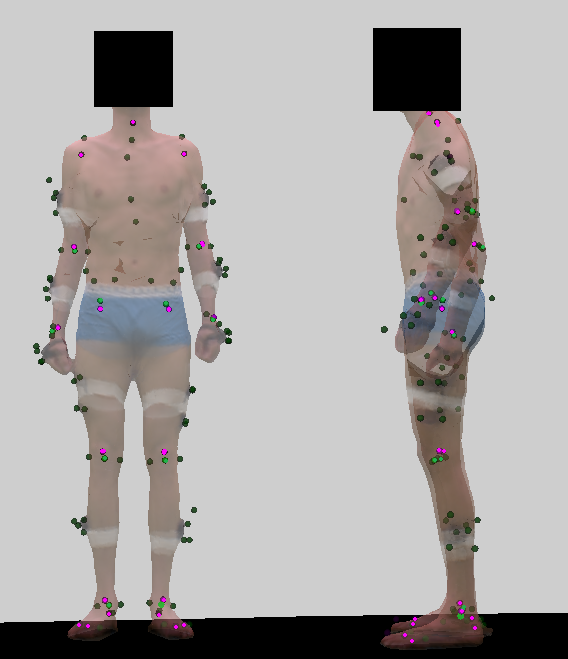
\includegraphics[width=\linewidth]{"../Chap3/Figures/Fig_MkMkl.png"}
	\caption{Triangulated anatomical markers and clusters (dark green), calculated joint centers (light green), and OpenPose body\_25b keypoints (pink) on a textured mesh. OpenPose’s eyes and ears keypoints were excluded. Mesh opacity was set to 0.5 in order to make all points visible. This view made it possible to precisely place OpenPose triangulated keypoints on the OpenSim model.}
	\label{fig_mkmkl}
\end{figure}

Scaling in OpenSim can be broken down into two parts: first, the proper scaling of the model, which adjusts bone dimensions and inertial properties according to the positions of the joint markers; second, the adjustment of the other markers on the model, especially anatomical and cluster markers. If the model is defined properly, there is no need for further marker adjustment on the model, since markers will not be subject to placement variation due to human error or to skin movement artifact. Each body is scaled according to a factor computed as a ratio of distances, defined by the distance between pairs of model markers over distance between corresponding pairs of experimental markers. The markers used for scaling are chosen as follows:

\clearpage

\begin{itemize}[itemsep=0em, topsep=0em, leftmargin=*]
      \item{Arm: distance between shoulder and elbow markers;}
      \item{Forearm: distance between elbow and wrist;}
      \item{Thigh: distance between hip and knee;}
      \item{Shank: distance between knee and ankle;}
      \item{Foot: distance between heel and big toe;}
      \item{Pelvis: distance between left and right hip;}
      \item{Torso: distance between neck and hip;}
      \item{Head: distance between head and nose;}
\end{itemize}
All weights of joint coordinates are set to 1, apart from those of the nose and the head, which are set to 0.2, and from those of the other head markers, which are set to 0. Since we process scaling during a T-pose, we add as a condition that ankle flexion should be fixed at a neutral 0° angle.

The inverse kinematic tool is used with the same marker weights as in the scaling step.

Unlike in marker-based capture, keypoints detection hardly depends on the operator, the subject, nor the context. For this reason, the scaling and the inverse kinematic steps are straightforward, and the provided setup files require little to no adjusting.


\section{Limitations and perspectives} \label{ch3_lim}

\subsection{Issues related to OpenPose}

Pose2Sim is currently primarily used with OpenPose as a 2D pose detection network. Despite it is very robust, it suffers from issues when used for full-body kinematic analysis. First, keypoint localization suffers from systematic offsets when compared to actual joint center positions \cite{Needham2021b}. Constraining these coordinates to a skeletal model largely reduces the detrimental impact of low-quality 2D joint center estimations. Nevertheless, these offsets have been taken into account in the provided OpenSim model, by shifting OpenPose keypoint placements with regard to marker-based calculated joint centers. This was done manually, but precisely, thanks to our overlayed view (see \nameref{sec:accuracy_methods} Chapter 5.2.) However, OpenPose’s offset may not be the same when a limb is extended as when it is bent, which may influence kinematic results on extreme poses, such as seen in some sports. Hence, using a 2D pose estimation model free from systematic biases on all ranges of motion would certainly improve kinematic accuracy. The body\_25b model is more accurate than the default body\_25 one, but it is still biased. 

Furthermore, both models only detect 25 keypoints. This makes inverse kinematics an under-constrained problem, which has to be guided with carefully chosen joint constraints, and with precise placement of markers on the model. Currently, all pelvis, lumbar, and thoracic angles are solely determined by the detection of the hip keypoints on the lower part, and of the shoulder and neck keypoints on the upper part. As a consequence, even if joint centers were perfectly estimated, the optimization procedure would admit two solutions for the spine curvature, both mathematically and kinematically correct: one with a lordotic posture, and the other with a kyphotic posture. Additionally, there is no marker for the hand, which does not allow for capture of any pronation/supination movement, let alone of any hand or finger movement. The shoulder is also defined as a ball joint, whereas the pectoral girdle is much more complex. Internal/external rotations are solved with difficulties despite the use of kinematic constraints. Using the experimental body\_135 OpenPose model would solve the hand issue, but it would also greatly increase the computational cost and would leave the shoulder and spine problem unaddressed. As a consequence, and provided that they are reliably labeled, OpenPose needs more keypoints to solve these indeterminations, and potentially several per joints, in the same way as markersets are designed in marker-based methods. Pose2Sim could operate with such a model, although new keypoints should then be placed afresh on the unscaled OpenSim model. 

Moreover, OpenPose struggles to accurately detect pose when the person is upside-down, or taking an unusual pose. One way to solve this is enhancing the OpenPose dataset, by augmenting it with larger rotations so that upside-down poses are recognized, or by training it on specific sports poses. One risk of this approach is that the model may perform better on specific extreme poses, but worse on standard ones \cite{Kitamura2022}. 

Another approach, which could solve altogether the offsets in labeling, the dearth of keypoints, and the lack of accuracy on sports poses, could be to train on a whole new dataset. Note that this dataset should not base its labeling on marker positions, which could be interpreted as visual cues, that are not available in real sports situations. However, this condition is not sufficient: the dataset should also be large and diverse enough, represent a wide variety of body types and of sports movements \cite{Seethapathi2019}, and include images with motion blur such as found in sports videos. One way to do it is to build a synthetic dataset. For example, a mass of c3D motion files could be gathered from various sports, and be used to fit an SMPL+H mesh \cite{Pavlakos2019} with AMASS \cite{Mahmood2019}. These data could be augmented with already existing datasets for daily life activities, such as Agora \cite{Patel2021}. Then, it would be possible to take advantage of the fact that the topology of an SMPL mesh is constant, and assume that only labelling the first frame of any given sequence should be sufficient: label positions should be consistently propagated to the next frames. At this stage, one could place as many virtual markers as needed, for a precise evaluation of any movement and pose. However, only an expert should perform this task, and make sure that markers are correctly positioned: crowd-sourcing this task, like it is done for more basic image classification and segmentation with ImageNet \cite{Deng2009}, has been proved to lead to systematic offset errors \cite{Needham2021b}. Finally, random clothing, background, and light could be added (see \cite{Wood2021,Bolanos2021} for a detailed workflow), as well as variations in SMPL shape parameters. The scene would be filmed with numerous virtual cameras, in order to gather a large amount of diverse perspectives, and virtual markers would be automatically projected on the camera planes. This would result in an extensive sports dataset, created with minimal labelling work, on a potentially infinite amount of views. Nevertheless, before training the network, one should make sure that the generated data is as diverse as the real world, by using one of the metrics proposed by \cite{Borji2019, Borji2022}. Additionally, keypoint positions need to be precise enough: SMPL shape vertices can sometimes be more than 5 cm apart, which could cause imprecision errors similar to skin artifacts. Besides, instead of constraining pose estimation results with a physically consistent skeletal model, it would be interesting to develop a physics-informed pose estimation model \cite{Raissi2019}, which would offer the opportunity of embedding the kinematics priors as early as possible in the learning process.

On a different note, in a sports context, not only the human pose is of interest: sports gear can also be considerably important to detect, such as a ball \cite{Ghasemzadeh2021}, skis \cite{Ludwig2020}, or bike parts in the context of cycling (see Chapter 7 on \hyperref[ch:7]{Joint OpenPose and DeepLabCut detection}). This can help to analyze game dynamics, and to quantify posture cues related to a specific sports discipline. This can be dones, for example, by separately process the video with OpenPose, as well as with a custom-trained DeepLabCut model. Resulting .trc coordinate files can be merged, and used in OpenSim. However, the DeeLabCut keypoints must be referenced on an OpenSim model, which may need to be crafted from scratch, such as a ball, skis, or bike, depending on the detected object.


\subsection{Multi-person analysis}

Pose2Sim has several limitations. First, despite it is not altered by people entering the field of view, it can currently only analyze the movement of one single person. For races, team sports, and combat sports, it would be useful to be able to analyze the movement of several athletes at the same time. This could be achieved in two steps: first, by triangulating all the persons whose reprojection error is below a certain threshold, instead of taking only the one with minimum error, in a similar way as carried out by \cite{Slembrouck2020}; then, by tracking the triangulated persons in time, e.g., by limiting the displacement speed of each person’s neck keypoint from one frame to the next one. Another way, probably faster, would be to compute affinity matrices for each detected persons in each view, and cluster all detected persons as individuals together \cite{Dong2019}. Or else, one could use a spatio-temporal neural network, which would take advantage of the information gathered in previous frames instead of working frame-by-frame \cite{Raaj2019}.


\subsection{User-friendly calibration}

Calibration remains a challenging task in daylight, at a distance, and with non research-grade cameras. It could be useful to make it more robust, either by implementing the Aniposelib library \cite{Karashchuk2020}, by importing calibration files from an Argus wand calibration \cite{Argus2017}, or by automatically calibrating on people’s limb length \cite{Liu2022a}. Along with synchronization of light-weight cameras, this topic will be detailed in Chapter 6 on \nameref{ch:6} \cite{Pagnon2022c}.


\subsection{Visualization tools}\label{subsec:viztools}

Pose2Sim does not provide a GUI yet. This can make it complicated for coaches to adopt the tool. However, the code has been adopted by other entities. The 3D animation "CEB" studio built a Blender \cite{Blender1998} extension using Pose2Sim for realistic 3D markerless animation. However, it is not free nor open-source \cite{Barreto2022} (Figure~\ref{fig_mpp2sos}). In addition, the CAMERA laboratory of the University of Bath is currently developing a GUI around Pose2Sim, which would make the tool more accessible. 

\begin{figure}[hbtp]
      \centering
      \def\svgwidth{1\columnwidth}
      \fontsize{10pt}{10pt}\selectfont
      \href{https://blendermarket.com/products/mocap-mpp2soss}{
            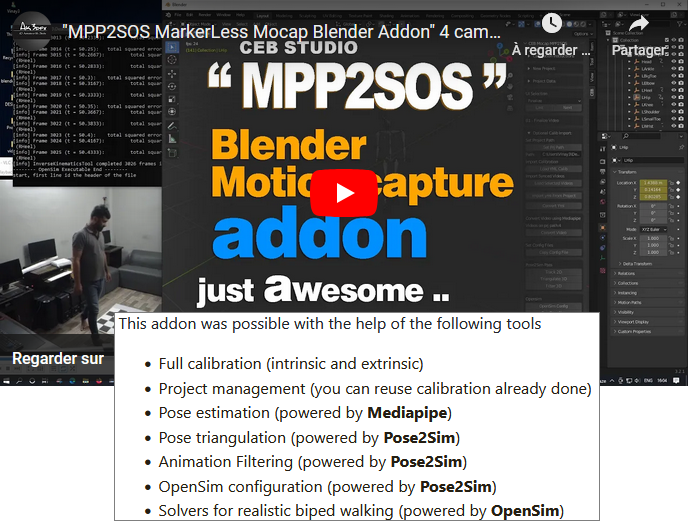
\includegraphics[width=0.93\linewidth]{"../Chap3/Figures/Fig_MPP2SOS.png"}
      }
      \caption{CEB Studio built the MPP2SOS Blender add-on, which uses Pose2Sim for realistic 3D markerless animation}
      \label{fig_mpp2sos}
\end{figure}

\begin{figure}[hbtp!]
	\centering
	\begin{subfigure}[b]{1\textwidth}
		\centering
		\def\svgwidth{\columnwidth}
		\fontsize{10pt}{10pt}\selectfont
		\href{https://github.com/davidpagnon/Maya-Mocap}{
                  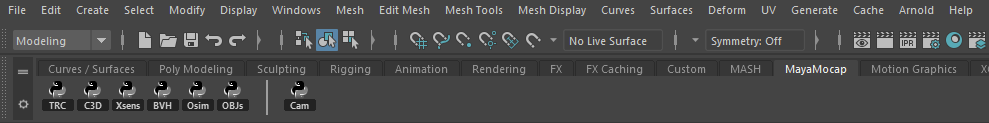
\includegraphics[width=\linewidth]{"../Chap3/Figures/Fig_MayaMocap1.png"}
            }
            \caption{The Maya-Mocap add-on is displayed as an additional toolbar in Maya.}
      \end{subfigure}
	\qquad
	\begin{subfigure}[b]{1\textwidth}
		\centering
		\def\svgwidth{\columnwidth}
		\fontsize{10pt}{10pt}\selectfont
		\href{https://github.com/davidpagnon/Maya-Mocap}{
                  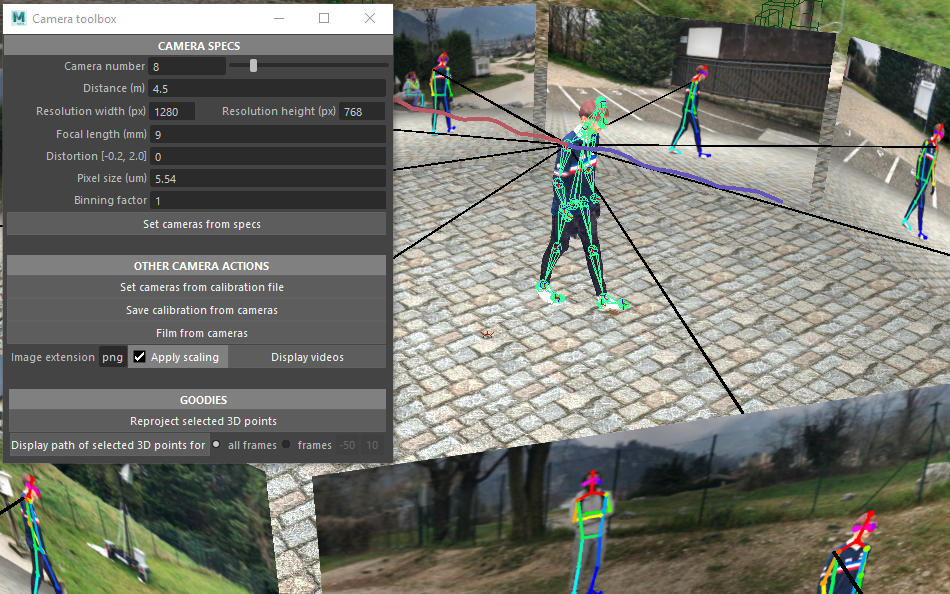
\includegraphics[width=\linewidth]{"../Chap3/Figures/Fig_MayaMocap2.png"}
            }
            \caption{Maya-Mocap can import several file types, e.g., a .trc motion file (bright green) or a textured animated 3D mesh. It can also load cameras from a calibration file, film with them, and display the filmed image sequences. In addition, it can reproject a selected point onto the camera plane (black lines), to make sure that it has been correctly triangulated. The 3D trajectory of a point can also be highlighted (red and blue lines).}
      \end{subfigure}
      \begin{subfigure}[b]{1\textwidth}
		\centering
		\def\svgwidth{\columnwidth}
		\fontsize{10pt}{10pt}\selectfont
            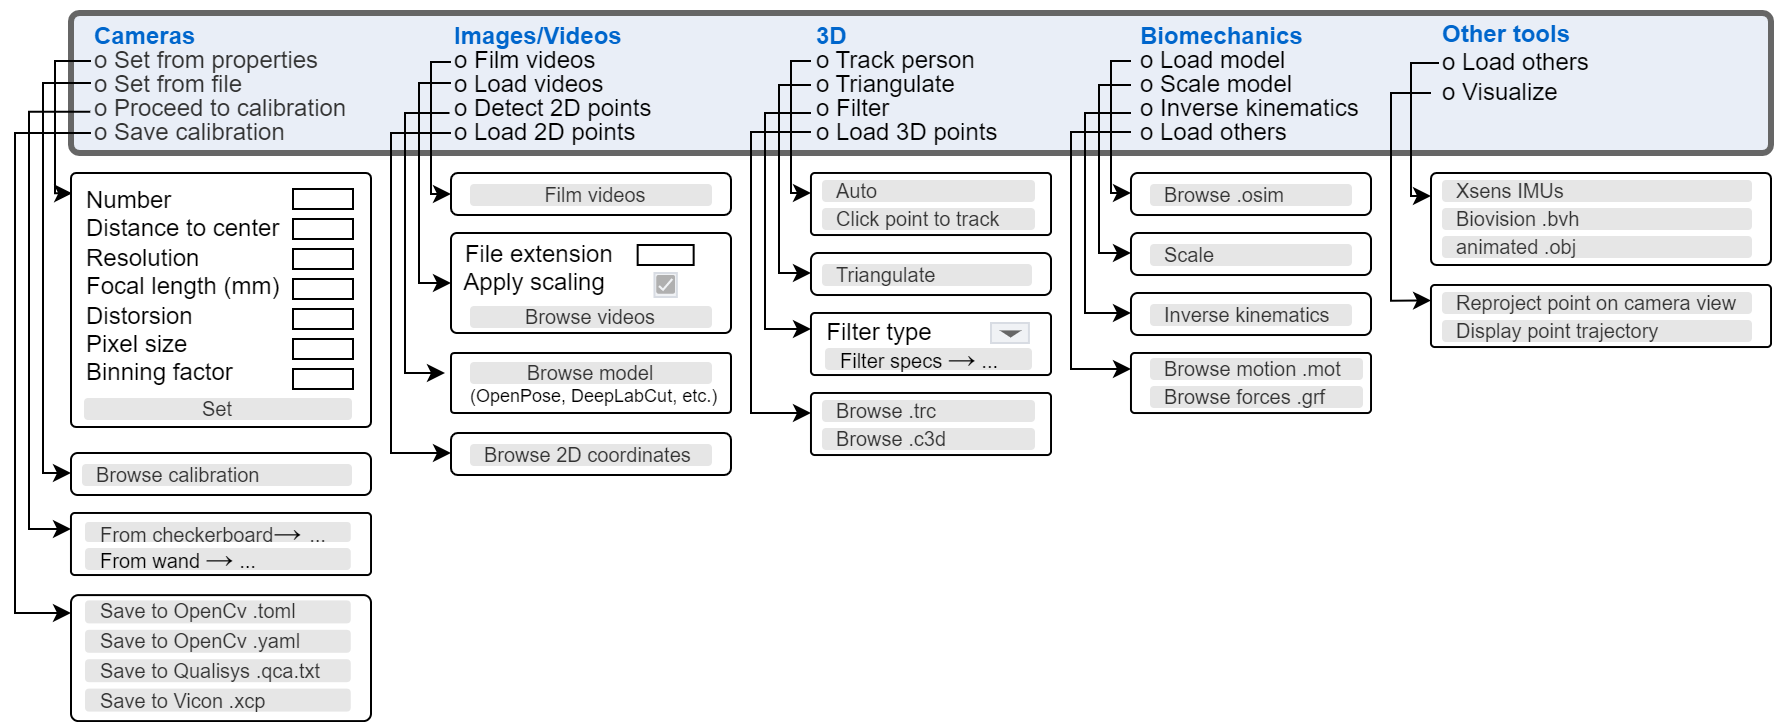
\includegraphics[width=\linewidth]{"../Chap3/Figures/Fig_MayaMocap3.png"}
            \caption{The organigram of Maya-Mocap planned abilities.}
      \end{subfigure}
 	\caption{The Maya-Mocap add-on (a-b), and the tool set that it should eventually provide (c).}
	\label{fig_mayamocap}
\end{figure}

I also developed a toolbox for Maya \cite{Maya1998} called Maya Mocap \cite{Pagnon2020}. First, it can import and display various types of motion files. Then, it can load cameras from a calibration file, film with them, and import the filmed image sequences. It can also help to make sure that triangulated points are well reprojected on the camera plane, by tracing a line from the point to the camera center. In addition, it can display the 3D trajectory of a point (see Figure~\ref{fig_mayamocap}). Next objectives would be to make it able to import an OpenSim model and its motion files, and to present it as a cleaner package, ready to be released. Since all the tools used in Pose2Sim are open-source, it would also be more consistent to translate it into Blender instead of Maya, in order to offer an entirely operational and open-source tool.


\subsection{Real-time analysis}\label{subsec:realtime}

Currently, Pose2Sim does not work in real time. This is a drawback for coaches and athletes, who need feedback in a timely manner. However, a timely analysis of athletes’ movements directly on the sports field appears to be achievable. Indeed, OpenPose is faster than most of its competitors \cite{Chen2020}, and the rest of the process is not computationally costly. Moreover, the pose detection, the triangulation, and the OpenSim inverse kinematic optimization work frame by frame. As a consequence, it is conceivable to calibrate and scale the model first, and then to feed the GUI frame by frame. This would allow the system to work only with a few seconds of delay.


\subsection{Other perspectives}

Other minor adjustments could be made in order to improve the triangulation and the filtering steps. Implementing Random Simple Consensus (RANSAC) triangulation \cite{Fischler1981} as an alternative to our weighted Direct Linear Transform (DLT) \cite{Pagnon2021}, and opting for optimal fixed-interval Kalman smoothing instead of low-pass filtering \cite{Rauch1965,Needham2021a}, may reduce errors, especially in large outliers. Performing the pose estimation, the triangulation, and the inverse kinematics on the cloud rather than on a local computer could allow athletes and coaches to use the software in a web application. Adding muscles which were stripped from the skeleton in the OpenSim model could allow for joint kinetics prediction. Neural networks could be trained to estimate ground reaction forces from kinetics on specific tasks, without the use of a force platform \cite{Oh2013,Johnson2018,Mundt2019}.
